%% amssamp1.tex is nearly identical to amssamp2.tex, except
%% that amssamp2.tex uses the [twocol] option to produce
%% two-column text.

%\documentclass{ametsoc}

\documentclass[twocol]{ametsoc}

%%%%%%%%%%%%%%%%%%%%%%%%%%%%%%%%
%%% To be entered only if twocol option is used

\journal{jtech}
\usepackage{graphicx}
\usepackage{caption}
\usepackage{subcaption}

%  Please choose a journal abbreviation to use above from the following list:
% 
%   jamc     (Journal of Applied Meteorology and Climatology)
%   jtech     (Journal of Atmospheric and Oceanic Technology)
%   jhm      (Journal of Hydrometeorology)
%   jpo     (Journal of Physical Oceanography)
%   jas      (Journal of Atmospheric Sciences)	
%   jcli      (Journal of Climate)
%   mwr      (Monthly Weather Review)
%   wcas      (Weather, Climate, and Society)
%   waf       (Weather and Forecasting)
%   bams (Bulletin of the American Meteorological Society)
%   ei    (Earth Interactions)

%%%%%%%%%%%%%%%%%%%%%%%%%%%%%%%%
%Citations should be of the form ``author year''  not ``author, year''
\bibpunct{(}{)}{;}{a}{}{,}

%%%%%%%%%%%%%%%%%%%%%%%%%%%%%%%%

\title{A report on progress on Corrected Moments in Antenna Coordinates 2.0}

\authors{Scott Collis\correspondingauthor{Scott Collis, Argonne National Laboratory, 
Environmental Science division, 
9700 South Cass Ave, Argonne, IL 60514} 
and Jonathan Helmus}

\affiliation{Environmental Science Division, Argonne National Laboratory} 

\email{scollis@anl.gov}

%\extraauthor{Extra Author}
%\extraaffil{Affiliation, City, State/Province, Country}



\abstract{In 2010 the Atmospheric Radiation Measurement program procured a number of 3 and 5cm wavelength radars for documenting the macrophysical, microphysical and dynamical structure of precipitating systems. In order to maximize the scientific impact the program supported the development of an application chain to correct for various phenomena in order to retrieve the "point" values of moments of the radar spectrum and polarimetric measurements. This report details the motivation, science and progress to date as well as charting a path forward.}

\begin{document}

\maketitle


\section{Introduction}
The Atmospheric Radiation Measurement Program (\cite{mather_arm_2012}) (ARM) has a long history of sensing clouds in the column using the Millimeter Cloud Radar (MMCR, Now Ka-Band Zenith Radar or KaZR). Starting in 2010 ARM embarked on program to better characterize the domain surrounding the column using scanning radars at millimeter and centimeter wavelengths. Processing for the shorter wavelengths has been previously published  \cite{kollias_scanning_2013} this report is limited to 5 and 3cm wavelengths. Due to the agility and lower cost per radar the program opted not to operate the common wavelength of 10cm (S-Band) which is  robust to liquid water path attenuation in all but the most severe storms. This necessitates the development of robust code for the correction of issues due to the two way propagation of the radar through medium that both scatters and attenuates. In addition, the trade off between wavelength, maximum unambiguous range and Doppler nyquist velocity means the radars alias at 12.4 and 16.52 $\mathrm{ms^{-1}}$ for 3 and 5cm respectively when operating in a baseline mode (such as during the Mid-Latitude  Convective Continental Clouds Experiment $\mathrm{MC^3E} $ (\cite{jensen_midlatitude_2015}). Due to extreme velocities of scatterers aloft and, in places such as Oklahoma, at the surface, aliasing is common and requires post moment calculation dealiasing. There are many techniques for dealiasing Doppler velocities (eg \cite{james_real-time_2001}) however on testing we found these techniques to be either difficult to implement in an operational chain or lacking in robustness. 

When we first attempted to build a processing chain each step made its own decision on where to conditionally run based on various measurements of "quality"  such as the co-polar (zero lag) correlation coefficient $\mathrm{\rho_{HV}}$ and Normalized Coherent Power (NCP, also referred to as Signal Quality Index or SQI). These are defined as:
\begin{align}
\rho_{HV}(0) &= \frac{|<S_{VV}S_{hh}^*>|}{\sqrt{<|S_{HH}|^2><|S_{VV}|^2>}}\\
NCP &= \frac{P_{coh}}{P_{DC}}.
\end{align}

Where the $S$ terms are elements of the scattering matrix, $P_{coh}$ is the coherent part of the doppler spectrum and $P_{DC}$ is the incoherent part. Since ARM radars use magnetron transmitters the phase is randomized from pulse to pulse so when a first trip return is mixed with a return from a scatterer beyond the maximum unambiguous range the derived radar Doppler spectrum when averaged over many pulses is flat and the NCP is low. While the Doppler spectrum from a first trip has structure from which (depending on the method) a peak can be found and Doppler velocity determined and the NCP approaches 1.0. However, the usefulness of NCP alone in second trip detection breaks down in regions of high spectral width. When the spectral width approaches the nyquist velocity, even in areas of purely first trip, the NCP decreases. This is especially troublesome in regions of high convergence and divergence in convective storms, often causing false flagging of these regions. 

To overcome the issues of arbitrary decision making and faults in using NCP alone to detect multiple trips our application chain, Corrected Moments in Antenna Coordinates first attempts to identify the nature of the scattering medium at the gate. This gate-ID is performed before any corrections are applied so it is different to hydrometeor identification codes (eg \cite{dolan_theory-based_2009}, \cite{wen_cluster-based_2015}, \cite{al-sakka_new_2013} etc.)


\section{Application chain}
Show the chain
\begin{figure}[h]
    \centering
    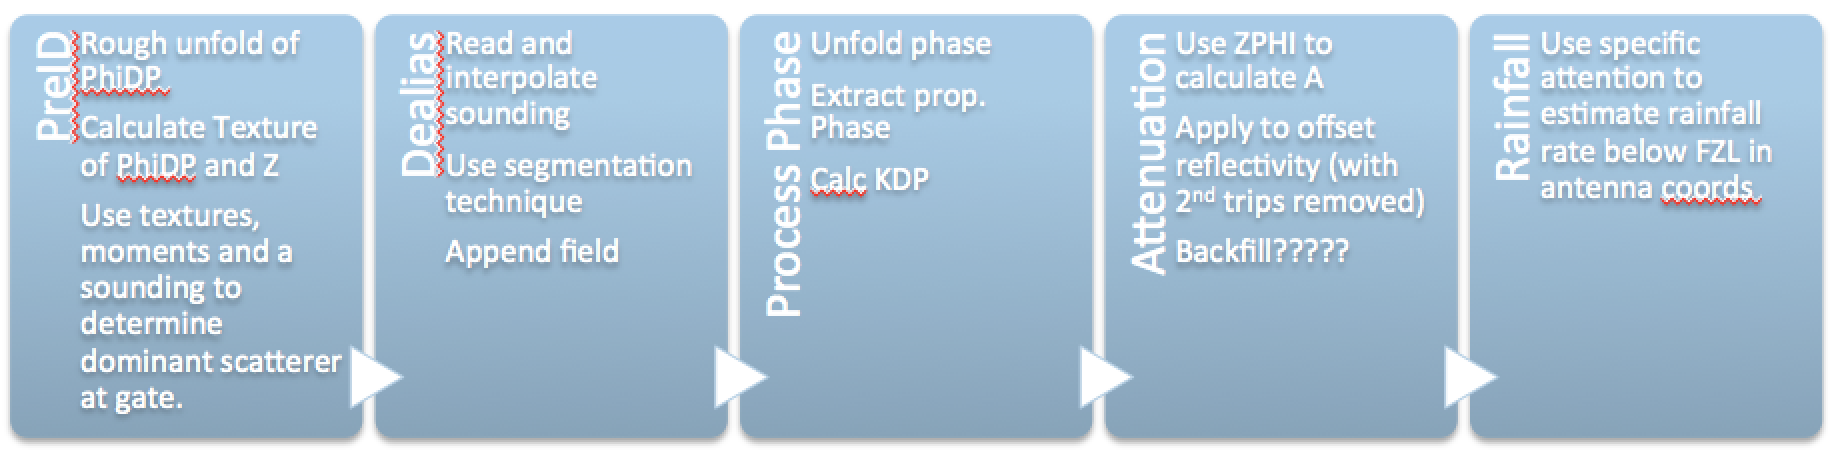
\includegraphics[width=0.9\columnwidth]{application_chain.png}
    \label{fig:chain}
    \caption{The Application chain for Corrections in Antenna Coordinates 2.0}
\end{figure}


\subsection{Calculations performed to aid identification of scatterers at gate}
Texture 
\begin{figure}[h]
    \centering
    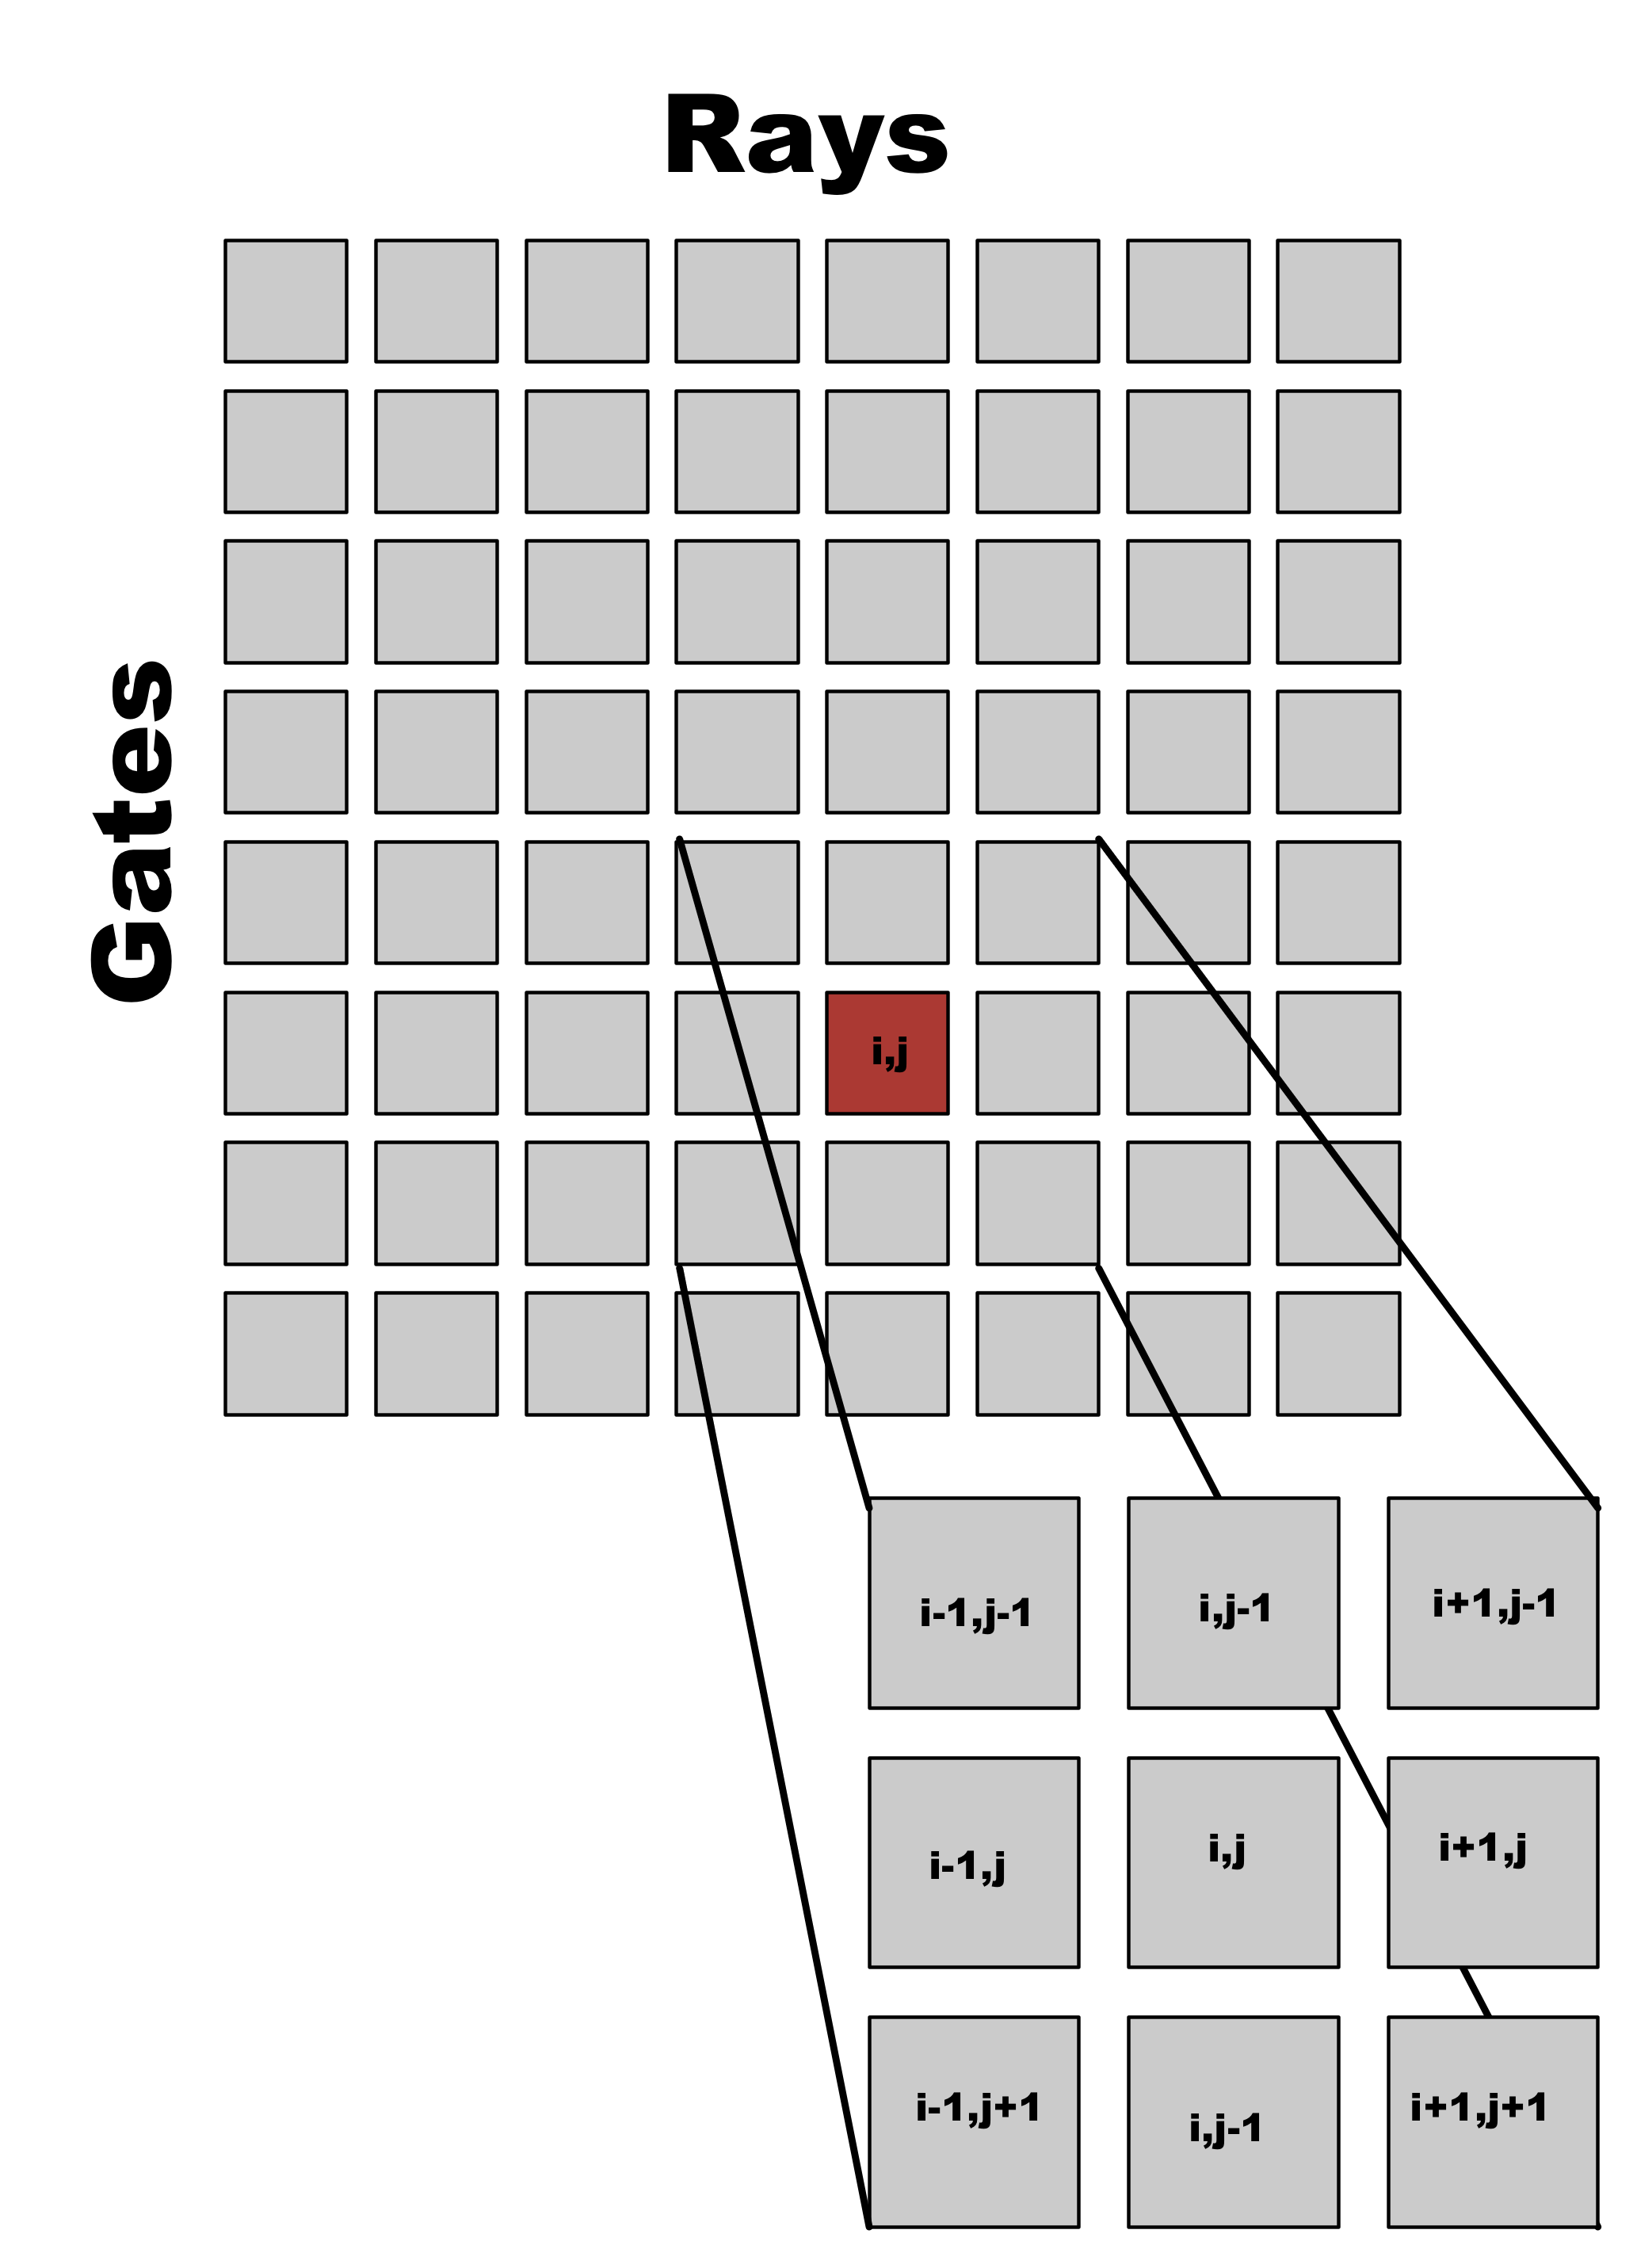
\includegraphics[width=0.6\columnwidth]{grid.png}
    \label{fig:grid}
    \caption{Illustration of the concept of a moving filter over range gates of adjacent rays. The center element, $\mathrm{(i,j)}$ is calculated by passing surrounding elements. The footprint of the surrounding elements is determined by the kernel. In many cases we use a 3x3 kernel}
\end{figure}

\begin{figure}[h]
    \centering
    \begin{subfigure}[b]{0.4\columnwidth}
        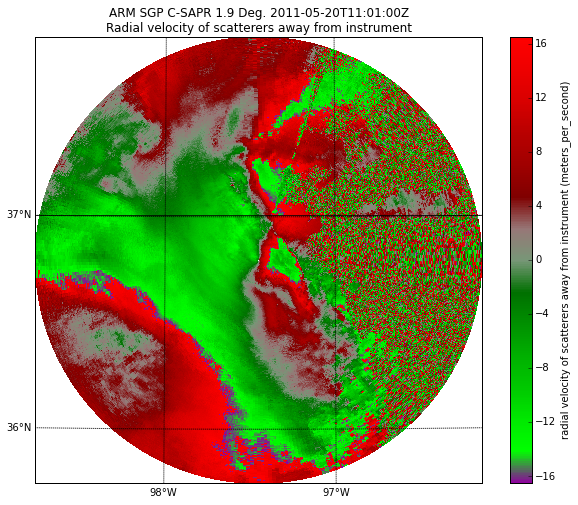
\includegraphics[width=\columnwidth]{radial_velocity.png}
        \caption{Radial velocity}
        \label{fig:textcalc:vr}
    \end{subfigure}
     %add desired spacing between images, e. g. ~, \quad, \qquad, \hfill etc. 
      %(or a blank line to force the subfigure onto a new line)
    \begin{subfigure}[b]{0.4\columnwidth}
        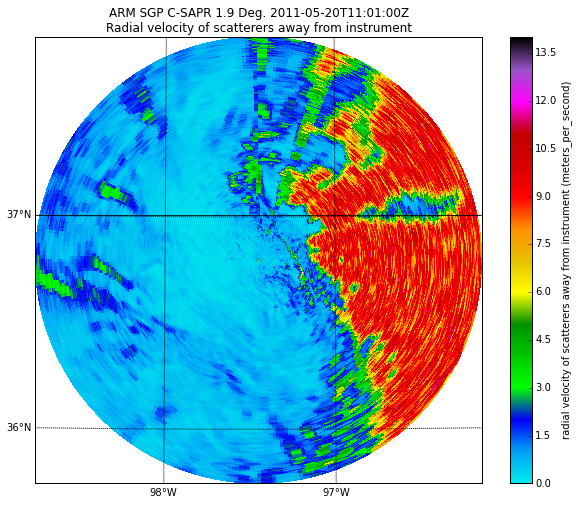
\includegraphics[width=\columnwidth]{texture.png}
        \caption{Texture}
        \label{fig:textcalc:vr}
    \end{subfigure}
    \caption{Calculations of texture of radial velocity from the C-Band Scanning ARM Precipitation Radar (C-SAPR) using circular statistic to avoid false texture on folds}\label{fig:textcalc}
\end{figure}
\subsubsection{Fuzzy logic based identification of scatterers at gate}
Cool stuff on Gate ID \cite{gourley_fuzzy_2007}


\section{Challeges}
The data u

\section{Future work}
The climatology and varianc

%%%%%%%%%%%%%%%%%
%ACKNOWLEDGMENTS
%%%%%%%%%%%%%%%%%

\acknowledgments{}

Scott G

Patricia

%%%%%%%%%%%%%%%%%
%APPENDIXES
%%%%%%%%%%%%%%%%%
%\appendix
%\appendixtitle{Appendix Title}
%
%\subsection*{Appendix section head}
%
%Here is a sample appendix.
%\begin{equation}
%\frac{
%pf \cos\phi}
%{p^0|\nabla h\bar q|(d\theta_0/dz)}
%\end{equation}
%
%\appendix[B]
%\appendixtitle{Second Appendix Title}
%\subsection{Sample appendix section head}
%Second appendix example.
%\subsection{Sample appendix section head}
%\begin{equation}
%\left(\frac{\partial\bar q}{\partial x}
%\overline{U'\theta'} +
%\frac{\partial\bar q}{\partial y}
%\overline{V'\theta'}\right) 
%\end{equation}


%%%%%%%%%%%%%%%%%
%REFERENCES
%%%%%%%%%%%%%%%%%

\bibliographystyle{ametsoc2014}
\bibliography{zotero}

%%%%%%%%%%%%%%%%%
% TABLES
%%%%%%%%%%%%%%%%%

%\begin{table}
%\caption{Percentage of variance explained by the first four
%EOFs for the North Pacific Bx. The degree of separation between
%EOF1 and EOF2 and EOF2 and EOF3, based on the North et al.
%(1982) criterion, is indicated by good (GD) and not good or marginal
%(NG).}
%\begin{tabular*}{\hsize}{@{\extracolsep\fill}lcccccc@{}}
%\topline
%Month& EOF1& Split &EOF2& Split& EOF3& EOF4\\
%\midline
%\ Jan& 29& NG& 24& GD& 10& 5\\
%\ Feb& 39& GD& 20& GD& \phantom{1}7 &6\\
%\ Mar& 31& GD& 14& NG& 10& 6\\
%\ Apr& 23& GD& 14& NG& 10& 7\\
%\ May& 19& GD& 12& NG& 10& 7\\
%\ Jun& 19& GD& 12& NG& 10& 9\\
%\ Jul& 18& NG &13& NG& \phantom{1}9& 7\\
%\ Aug& 18& NG& 13& NG& 11& 9\\
%\ Sep &17& NG& 13& NG& 10& 8\\
%\ Oct &16& NG& 13& GD& \phantom{1}8& 7\\
%\ Nov &19 &NG& 16& NG& 11& 8\\
%\ Dec& 33& GD& 18& GD& 10& 6\\
%\botline
%\end{tabular*}
%\end{table}

%
%
%\begin{table}
%\centering
%\caption{Years selected for anomaly composites for the positive
%phase of $B^x$ EOF1.}
%\begin{tabular}{lc}
%\topline
%Month& Yr of positive phase\\
%\midline
%\ \ Jan& 1961, 1969, 1978, 1979, 1988, 1990, 1992, 1994\\
%\ \ Feb& 1964, 1977, 1978, 1980, 1983, 1986, 1988, 2000, 2001\\
%\ \ Mar& 1970, 1973, 1979, 1980, 1984, 1988, 2000\\
%\ \ Apr& 1959, 1961, 1962, 1963, 1968, 1972, 1983, 2002\\
%\ \ May& 1971, 1984, 1993, 1996, 2000\\
%\ \ Jun& 1981, 1983, 1984, 1993, 1998\\
%\ \ Jul& 1961, 1972, 1973, 1978, 1994, 2000\\
%\ \ Aug& 1967, 1970, 1973, 1978, 1994, 1999\\
%\ \ Sep& 1975, 1977, 1988, 1989, 1994, 1998, 1999\\
%\ \ Oct& 1962, 1977, 1998, 1999, 2001\\
%\ \ Nov& 1985, 1986, 1987, 1988, 1991, 1998\\
%\ \ Dec& 1957, 1968, 1972, 1978, 1979, 1990\\
%\botline
%\end{tabular}
%\end{table}
%
%\begin{table}
%\centering
%\caption{Years selected for anomaly composites for the negative
%phase of $B^x$ EOF1.}
%\begin{tabular}{lc}
%\topline
%Month& Yr of negative phase\\
%\midline
%\ \ Jan&1962, 1963, 1968, 1974, 1991, 1996, 1997\\
%\ \ Feb& 1959, 1963, 1971, 1974, 1976, 1979, 1985, 1989, 1990, 1994\\
%\ \ Mar& 1963, 1968, 1972\\
%\ \ Apr& 1984, 1988, 1993, 1996, 1999, 2000\\
%\ \ May& 1961, 1963, 1983, 1987, 1997\\
%\ \ Jun& 1961, 1972, 1978, 1980, 1982, 1986\\
%\ \ Jul& 1964, 1974, 1980, 1983, 1986, 1988, 1993\\
%\ \ Aug& 1980, 1987, 1991, 1993, 1997\\
%\ \ Sep& 1959, 1963, 1969, 1983, 1985, 1993\\
%\ \ Oct& 1957, 1986, 1993, 1996, 1997\\
%\ \ Nov& 1958, 1968, 1970, 1982, 1997\\
%\ \ Dec& 1969, 1974, 1976, 1985, 1998, 1999, 2000, 2001\\
%\botline
%\end{tabular}
%\end{table}

%%%%%%%%%%%%%%%%%
% FIGURES
%%%%%%%%%%%%%%%%%

%\begin{figure}[t]
%\centerline{\includegraphics[width=\textwidth]{figone.pdf}}
%
%\caption{Climatology of $Bx (10^{-6} s^{-1}$, color) and $U^{200}$(m s$^-1$,
%contours) for (a) February and (b) August; $\overline{V'\theta'}^{850}$
%(K m s$^-1$, color) and 
%$\overline{V'V'}^{200}$
%(m$^2$ s$^{-1}$, contours) for (c) February and (d) August; MR$^{z850}$ 
%(10$^{-3}$ m$^2$ s$-2$, color) and $U^{1000}$ (m s$^{-1}$, contours) 
%for (e) February and (f) August;
%and SST (K, color) and $F_h$ [10$^5$ J m$^{-2}$ (6 h)$^{-1}$] for (g)
%February and (h) August. Red rectangles indicate the domain of EOF
%calculations.} \label{fig1} 
%\end{figure}
%
%\begin{figure}[p]
%\centerline{\includegraphics{FigTwo.pdf}}
%\caption{As in Fig.~10, but for (a),(b) September EOF1; (c),(d) September EOF2; (e),(f) October EOF1; (g),(h) October EOF2; and
%(i),(j) December EOF2.}
%\end{figure}
%
%\begin{figure}
% \centerline{\includegraphics[width=19pc]{figure01.pdf}}
%\appendcaption{A1}{Here is an appendix, single column figure caption.}
%\end{figure}
%



\end{document}





